% Created by tikzDevice version 0.12.6 on 2025-02-11 03:44:01
% !TEX encoding = UTF-8 Unicode
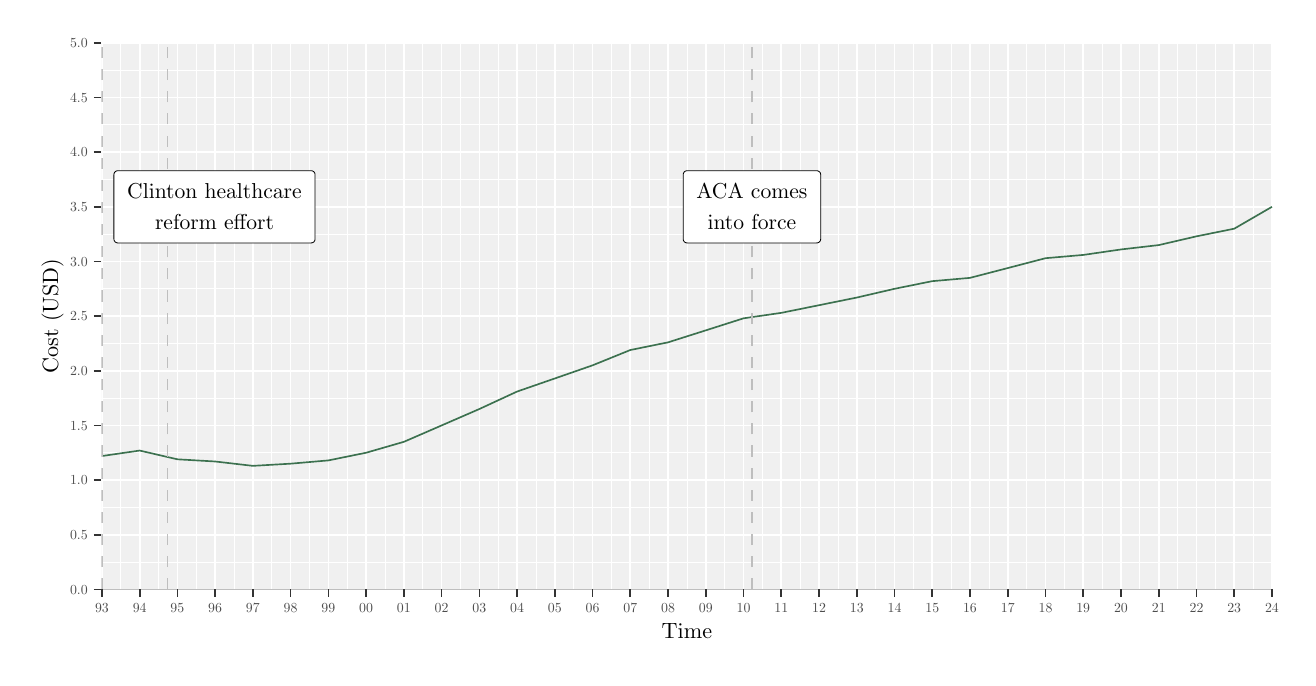
\begin{tikzpicture}[x=1pt,y=1pt]
\definecolor{fillColor}{RGB}{255,255,255}
\path[use as bounding box,fill=fillColor,fill opacity=0.00] (0,0) rectangle (455.30,227.65);
\begin{scope}
\path[clip] (  0.00,  0.00) rectangle (455.30,227.65);
\definecolor{drawColor}{RGB}{255,255,255}
\definecolor{fillColor}{RGB}{255,255,255}

\path[draw=drawColor,line width= 0.6pt,line join=round,line cap=round,fill=fillColor] (  0.00,  0.00) rectangle (455.30,227.65);
\end{scope}
\begin{scope}
\path[clip] ( 26.65, 24.68) rectangle (449.80,222.15);
\definecolor{fillColor}{gray}{0.94}

\path[fill=fillColor] ( 26.65, 24.68) rectangle (449.80,222.15);
\definecolor{drawColor}{RGB}{255,255,255}

\path[draw=drawColor,line width= 0.3pt,line join=round] ( 26.65, 34.55) --
	(449.80, 34.55);

\path[draw=drawColor,line width= 0.3pt,line join=round] ( 26.65, 54.30) --
	(449.80, 54.30);

\path[draw=drawColor,line width= 0.3pt,line join=round] ( 26.65, 74.05) --
	(449.80, 74.05);

\path[draw=drawColor,line width= 0.3pt,line join=round] ( 26.65, 93.80) --
	(449.80, 93.80);

\path[draw=drawColor,line width= 0.3pt,line join=round] ( 26.65,113.54) --
	(449.80,113.54);

\path[draw=drawColor,line width= 0.3pt,line join=round] ( 26.65,133.29) --
	(449.80,133.29);

\path[draw=drawColor,line width= 0.3pt,line join=round] ( 26.65,153.04) --
	(449.80,153.04);

\path[draw=drawColor,line width= 0.3pt,line join=round] ( 26.65,172.78) --
	(449.80,172.78);

\path[draw=drawColor,line width= 0.3pt,line join=round] ( 26.65,192.53) --
	(449.80,192.53);

\path[draw=drawColor,line width= 0.3pt,line join=round] ( 26.65,212.28) --
	(449.80,212.28);

\path[draw=drawColor,line width= 0.3pt,line join=round] ( 33.65, 24.68) --
	( 33.65,222.15);

\path[draw=drawColor,line width= 0.3pt,line join=round] ( 47.28, 24.68) --
	( 47.28,222.15);

\path[draw=drawColor,line width= 0.3pt,line join=round] ( 60.91, 24.68) --
	( 60.91,222.15);

\path[draw=drawColor,line width= 0.3pt,line join=round] ( 74.56, 24.68) --
	( 74.56,222.15);

\path[draw=drawColor,line width= 0.3pt,line join=round] ( 88.21, 24.68) --
	( 88.21,222.15);

\path[draw=drawColor,line width= 0.3pt,line join=round] (101.84, 24.68) --
	(101.84,222.15);

\path[draw=drawColor,line width= 0.3pt,line join=round] (115.47, 24.68) --
	(115.47,222.15);

\path[draw=drawColor,line width= 0.3pt,line join=round] (129.12, 24.68) --
	(129.12,222.15);

\path[draw=drawColor,line width= 0.3pt,line join=round] (142.76, 24.68) --
	(142.76,222.15);

\path[draw=drawColor,line width= 0.3pt,line join=round] (156.39, 24.68) --
	(156.39,222.15);

\path[draw=drawColor,line width= 0.3pt,line join=round] (170.02, 24.68) --
	(170.02,222.15);

\path[draw=drawColor,line width= 0.3pt,line join=round] (183.67, 24.68) --
	(183.67,222.15);

\path[draw=drawColor,line width= 0.3pt,line join=round] (197.32, 24.68) --
	(197.32,222.15);

\path[draw=drawColor,line width= 0.3pt,line join=round] (210.95, 24.68) --
	(210.95,222.15);

\path[draw=drawColor,line width= 0.3pt,line join=round] (224.58, 24.68) --
	(224.58,222.15);

\path[draw=drawColor,line width= 0.3pt,line join=round] (238.23, 24.68) --
	(238.23,222.15);

\path[draw=drawColor,line width= 0.3pt,line join=round] (251.87, 24.68) --
	(251.87,222.15);

\path[draw=drawColor,line width= 0.3pt,line join=round] (265.50, 24.68) --
	(265.50,222.15);

\path[draw=drawColor,line width= 0.3pt,line join=round] (279.13, 24.68) --
	(279.13,222.15);

\path[draw=drawColor,line width= 0.3pt,line join=round] (292.78, 24.68) --
	(292.78,222.15);

\path[draw=drawColor,line width= 0.3pt,line join=round] (306.43, 24.68) --
	(306.43,222.15);

\path[draw=drawColor,line width= 0.3pt,line join=round] (320.06, 24.68) --
	(320.06,222.15);

\path[draw=drawColor,line width= 0.3pt,line join=round] (333.69, 24.68) --
	(333.69,222.15);

\path[draw=drawColor,line width= 0.3pt,line join=round] (347.34, 24.68) --
	(347.34,222.15);

\path[draw=drawColor,line width= 0.3pt,line join=round] (360.99, 24.68) --
	(360.99,222.15);

\path[draw=drawColor,line width= 0.3pt,line join=round] (374.61, 24.68) --
	(374.61,222.15);

\path[draw=drawColor,line width= 0.3pt,line join=round] (388.24, 24.68) --
	(388.24,222.15);

\path[draw=drawColor,line width= 0.3pt,line join=round] (401.89, 24.68) --
	(401.89,222.15);

\path[draw=drawColor,line width= 0.3pt,line join=round] (415.54, 24.68) --
	(415.54,222.15);

\path[draw=drawColor,line width= 0.3pt,line join=round] (429.17, 24.68) --
	(429.17,222.15);

\path[draw=drawColor,line width= 0.3pt,line join=round] (442.80, 24.68) --
	(442.80,222.15);

\path[draw=drawColor,line width= 0.6pt,line join=round] ( 26.65, 24.68) --
	(449.80, 24.68);

\path[draw=drawColor,line width= 0.6pt,line join=round] ( 26.65, 44.43) --
	(449.80, 44.43);

\path[draw=drawColor,line width= 0.6pt,line join=round] ( 26.65, 64.17) --
	(449.80, 64.17);

\path[draw=drawColor,line width= 0.6pt,line join=round] ( 26.65, 83.92) --
	(449.80, 83.92);

\path[draw=drawColor,line width= 0.6pt,line join=round] ( 26.65,103.67) --
	(449.80,103.67);

\path[draw=drawColor,line width= 0.6pt,line join=round] ( 26.65,123.42) --
	(449.80,123.42);

\path[draw=drawColor,line width= 0.6pt,line join=round] ( 26.65,143.16) --
	(449.80,143.16);

\path[draw=drawColor,line width= 0.6pt,line join=round] ( 26.65,162.91) --
	(449.80,162.91);

\path[draw=drawColor,line width= 0.6pt,line join=round] ( 26.65,182.66) --
	(449.80,182.66);

\path[draw=drawColor,line width= 0.6pt,line join=round] ( 26.65,202.40) --
	(449.80,202.40);

\path[draw=drawColor,line width= 0.6pt,line join=round] ( 26.65,222.15) --
	(449.80,222.15);

\path[draw=drawColor,line width= 0.6pt,line join=round] ( 26.84, 24.68) --
	( 26.84,222.15);

\path[draw=drawColor,line width= 0.6pt,line join=round] ( 40.47, 24.68) --
	( 40.47,222.15);

\path[draw=drawColor,line width= 0.6pt,line join=round] ( 54.10, 24.68) --
	( 54.10,222.15);

\path[draw=drawColor,line width= 0.6pt,line join=round] ( 67.73, 24.68) --
	( 67.73,222.15);

\path[draw=drawColor,line width= 0.6pt,line join=round] ( 81.39, 24.68) --
	( 81.39,222.15);

\path[draw=drawColor,line width= 0.6pt,line join=round] ( 95.02, 24.68) --
	( 95.02,222.15);

\path[draw=drawColor,line width= 0.6pt,line join=round] (108.65, 24.68) --
	(108.65,222.15);

\path[draw=drawColor,line width= 0.6pt,line join=round] (122.28, 24.68) --
	(122.28,222.15);

\path[draw=drawColor,line width= 0.6pt,line join=round] (135.95, 24.68) --
	(135.95,222.15);

\path[draw=drawColor,line width= 0.6pt,line join=round] (149.58, 24.68) --
	(149.58,222.15);

\path[draw=drawColor,line width= 0.6pt,line join=round] (163.21, 24.68) --
	(163.21,222.15);

\path[draw=drawColor,line width= 0.6pt,line join=round] (176.84, 24.68) --
	(176.84,222.15);

\path[draw=drawColor,line width= 0.6pt,line join=round] (190.50, 24.68) --
	(190.50,222.15);

\path[draw=drawColor,line width= 0.6pt,line join=round] (204.13, 24.68) --
	(204.13,222.15);

\path[draw=drawColor,line width= 0.6pt,line join=round] (217.76, 24.68) --
	(217.76,222.15);

\path[draw=drawColor,line width= 0.6pt,line join=round] (231.39, 24.68) --
	(231.39,222.15);

\path[draw=drawColor,line width= 0.6pt,line join=round] (245.06, 24.68) --
	(245.06,222.15);

\path[draw=drawColor,line width= 0.6pt,line join=round] (258.69, 24.68) --
	(258.69,222.15);

\path[draw=drawColor,line width= 0.6pt,line join=round] (272.32, 24.68) --
	(272.32,222.15);

\path[draw=drawColor,line width= 0.6pt,line join=round] (285.95, 24.68) --
	(285.95,222.15);

\path[draw=drawColor,line width= 0.6pt,line join=round] (299.62, 24.68) --
	(299.62,222.15);

\path[draw=drawColor,line width= 0.6pt,line join=round] (313.24, 24.68) --
	(313.24,222.15);

\path[draw=drawColor,line width= 0.6pt,line join=round] (326.87, 24.68) --
	(326.87,222.15);

\path[draw=drawColor,line width= 0.6pt,line join=round] (340.50, 24.68) --
	(340.50,222.15);

\path[draw=drawColor,line width= 0.6pt,line join=round] (354.17, 24.68) --
	(354.17,222.15);

\path[draw=drawColor,line width= 0.6pt,line join=round] (367.80, 24.68) --
	(367.80,222.15);

\path[draw=drawColor,line width= 0.6pt,line join=round] (381.43, 24.68) --
	(381.43,222.15);

\path[draw=drawColor,line width= 0.6pt,line join=round] (395.06, 24.68) --
	(395.06,222.15);

\path[draw=drawColor,line width= 0.6pt,line join=round] (408.73, 24.68) --
	(408.73,222.15);

\path[draw=drawColor,line width= 0.6pt,line join=round] (422.36, 24.68) --
	(422.36,222.15);

\path[draw=drawColor,line width= 0.6pt,line join=round] (435.98, 24.68) --
	(435.98,222.15);

\path[draw=drawColor,line width= 0.6pt,line join=round] (449.61, 24.68) --
	(449.61,222.15);
\definecolor{drawColor}{RGB}{190,190,190}

\path[draw=drawColor,line width= 0.6pt,line join=round] ( 26.65, 24.68) -- (449.80, 24.68);
\definecolor{drawColor}{RGB}{60,113,79}

\path[draw=drawColor,line width= 0.6pt,line join=round] ( 26.84, 72.86) --
	( 40.47, 74.84) --
	( 54.10, 71.68) --
	( 67.73, 70.89) --
	( 81.39, 69.31) --
	( 95.02, 70.10) --
	(108.65, 71.28) --
	(122.28, 74.05) --
	(135.95, 78.00) --
	(149.58, 83.92) --
	(163.21, 89.85) --
	(176.84, 96.16) --
	(190.50,100.90) --
	(204.13,105.64) --
	(217.76,111.17) --
	(231.39,113.94) --
	(245.06,118.28) --
	(258.69,122.63) --
	(272.32,124.60) --
	(285.95,127.36) --
	(299.62,130.13) --
	(313.24,133.29) --
	(326.87,136.05) --
	(340.50,137.24) --
	(354.17,140.79) --
	(367.80,144.35) --
	(381.43,145.53) --
	(395.06,147.51) --
	(408.73,149.09) --
	(422.36,152.25) --
	(435.98,155.01) --
	(449.61,162.91);
\definecolor{drawColor}{RGB}{190,190,190}

\path[draw=drawColor,line width= 0.6pt,dash pattern=on 4pt off 4pt ,line join=round] (261.71, 24.68) -- (261.71,222.15);

\path[draw=drawColor,line width= 0.6pt,dash pattern=on 4pt off 4pt ,line join=round] ( 26.84, 24.68) -- ( 26.84,222.15);

\path[draw=drawColor,line width= 0.6pt,dash pattern=on 4pt off 4pt ,line join=round] ( 50.48, 24.68) -- ( 50.48,222.15);
\definecolor{drawColor}{RGB}{0,0,0}
\definecolor{fillColor}{RGB}{255,255,255}

\path[draw=drawColor,line width= 0.3pt,line join=round,line cap=round,fill=fillColor] ( 32.58,149.87) --
	(102.43,149.87) --
	(102.37,149.87) --
	(102.60,149.88) --
	(102.82,149.92) --
	(103.04,150.01) --
	(103.23,150.12) --
	(103.41,150.26) --
	(103.56,150.43) --
	(103.68,150.63) --
	(103.77,150.83) --
	(103.83,151.06) --
	(103.84,151.28) --
	(103.84,151.28) --
	(103.84,174.54) --
	(103.84,174.54) --
	(103.83,174.76) --
	(103.77,174.98) --
	(103.68,175.19) --
	(103.56,175.39) --
	(103.41,175.56) --
	(103.23,175.70) --
	(103.04,175.81) --
	(102.82,175.89) --
	(102.60,175.94) --
	(102.43,175.95) --
	( 32.58,175.95) --
	( 32.75,175.94) --
	( 32.52,175.95) --
	( 32.29,175.92) --
	( 32.07,175.86) --
	( 31.87,175.76) --
	( 31.68,175.63) --
	( 31.52,175.47) --
	( 31.38,175.29) --
	( 31.27,175.09) --
	( 31.20,174.87) --
	( 31.17,174.65) --
	( 31.16,174.54) --
	( 31.16,151.28) --
	( 31.17,151.40) --
	( 31.17,151.17) --
	( 31.20,150.94) --
	( 31.27,150.73) --
	( 31.38,150.53) --
	( 31.52,150.35) --
	( 31.68,150.19) --
	( 31.87,150.06) --
	( 32.07,149.96) --
	( 32.29,149.90) --
	( 32.52,149.87) --
	cycle;
\end{scope}
\begin{scope}
\path[clip] ( 26.65, 24.68) rectangle (449.80,222.15);
\definecolor{drawColor}{RGB}{0,0,0}

\node[text=drawColor,anchor=base,inner sep=0pt, outer sep=0pt, scale=  0.78] at ( 67.50,165.85) {Clinton healthcare };

\node[text=drawColor,anchor=base,inner sep=0pt, outer sep=0pt, scale=  0.78] at ( 67.50,154.58) { reform effort};
\end{scope}
\begin{scope}
\path[clip] ( 26.65, 24.68) rectangle (449.80,222.15);
\definecolor{drawColor}{RGB}{0,0,0}
\definecolor{fillColor}{RGB}{255,255,255}

\path[draw=drawColor,line width= 0.3pt,line join=round,line cap=round,fill=fillColor] (238.29,149.87) --
	(285.14,149.87) --
	(285.08,149.87) --
	(285.31,149.88) --
	(285.53,149.92) --
	(285.74,150.01) --
	(285.94,150.12) --
	(286.11,150.26) --
	(286.27,150.43) --
	(286.39,150.63) --
	(286.48,150.83) --
	(286.53,151.06) --
	(286.55,151.28) --
	(286.55,151.28) --
	(286.55,174.54) --
	(286.55,174.54) --
	(286.53,174.76) --
	(286.48,174.98) --
	(286.39,175.19) --
	(286.27,175.39) --
	(286.11,175.56) --
	(285.94,175.70) --
	(285.74,175.81) --
	(285.53,175.89) --
	(285.31,175.94) --
	(285.14,175.95) --
	(238.29,175.95) --
	(238.46,175.94) --
	(238.24,175.95) --
	(238.01,175.92) --
	(237.79,175.86) --
	(237.59,175.76) --
	(237.40,175.63) --
	(237.23,175.47) --
	(237.10,175.29) --
	(236.99,175.09) --
	(236.92,174.87) --
	(236.88,174.65) --
	(236.88,174.54) --
	(236.88,151.28) --
	(236.88,151.40) --
	(236.88,151.17) --
	(236.92,150.94) --
	(236.99,150.73) --
	(237.10,150.53) --
	(237.23,150.35) --
	(237.40,150.19) --
	(237.59,150.06) --
	(237.79,149.96) --
	(238.01,149.90) --
	(238.24,149.87) --
	cycle;
\end{scope}
\begin{scope}
\path[clip] ( 26.65, 24.68) rectangle (449.80,222.15);
\definecolor{drawColor}{RGB}{0,0,0}

\node[text=drawColor,anchor=base,inner sep=0pt, outer sep=0pt, scale=  0.78] at (261.71,165.85) {ACA comes };

\node[text=drawColor,anchor=base,inner sep=0pt, outer sep=0pt, scale=  0.78] at (261.71,154.58) { into force};
\end{scope}
\begin{scope}
\path[clip] (  0.00,  0.00) rectangle (455.30,227.65);
\definecolor{drawColor}{gray}{0.30}

\node[text=drawColor,anchor=base east,inner sep=0pt, outer sep=0pt, scale=  0.50] at ( 21.70, 22.96) {0.0};

\node[text=drawColor,anchor=base east,inner sep=0pt, outer sep=0pt, scale=  0.50] at ( 21.70, 42.71) {0.5};

\node[text=drawColor,anchor=base east,inner sep=0pt, outer sep=0pt, scale=  0.50] at ( 21.70, 62.45) {1.0};

\node[text=drawColor,anchor=base east,inner sep=0pt, outer sep=0pt, scale=  0.50] at ( 21.70, 82.20) {1.5};

\node[text=drawColor,anchor=base east,inner sep=0pt, outer sep=0pt, scale=  0.50] at ( 21.70,101.95) {2.0};

\node[text=drawColor,anchor=base east,inner sep=0pt, outer sep=0pt, scale=  0.50] at ( 21.70,121.69) {2.5};

\node[text=drawColor,anchor=base east,inner sep=0pt, outer sep=0pt, scale=  0.50] at ( 21.70,141.44) {3.0};

\node[text=drawColor,anchor=base east,inner sep=0pt, outer sep=0pt, scale=  0.50] at ( 21.70,161.19) {3.5};

\node[text=drawColor,anchor=base east,inner sep=0pt, outer sep=0pt, scale=  0.50] at ( 21.70,180.93) {4.0};

\node[text=drawColor,anchor=base east,inner sep=0pt, outer sep=0pt, scale=  0.50] at ( 21.70,200.68) {4.5};

\node[text=drawColor,anchor=base east,inner sep=0pt, outer sep=0pt, scale=  0.50] at ( 21.70,220.43) {5.0};
\end{scope}
\begin{scope}
\path[clip] (  0.00,  0.00) rectangle (455.30,227.65);
\definecolor{drawColor}{gray}{0.20}

\path[draw=drawColor,line width= 0.6pt,line join=round] ( 23.90, 24.68) --
	( 26.65, 24.68);

\path[draw=drawColor,line width= 0.6pt,line join=round] ( 23.90, 44.43) --
	( 26.65, 44.43);

\path[draw=drawColor,line width= 0.6pt,line join=round] ( 23.90, 64.17) --
	( 26.65, 64.17);

\path[draw=drawColor,line width= 0.6pt,line join=round] ( 23.90, 83.92) --
	( 26.65, 83.92);

\path[draw=drawColor,line width= 0.6pt,line join=round] ( 23.90,103.67) --
	( 26.65,103.67);

\path[draw=drawColor,line width= 0.6pt,line join=round] ( 23.90,123.42) --
	( 26.65,123.42);

\path[draw=drawColor,line width= 0.6pt,line join=round] ( 23.90,143.16) --
	( 26.65,143.16);

\path[draw=drawColor,line width= 0.6pt,line join=round] ( 23.90,162.91) --
	( 26.65,162.91);

\path[draw=drawColor,line width= 0.6pt,line join=round] ( 23.90,182.66) --
	( 26.65,182.66);

\path[draw=drawColor,line width= 0.6pt,line join=round] ( 23.90,202.40) --
	( 26.65,202.40);

\path[draw=drawColor,line width= 0.6pt,line join=round] ( 23.90,222.15) --
	( 26.65,222.15);
\end{scope}
\begin{scope}
\path[clip] (  0.00,  0.00) rectangle (455.30,227.65);
\definecolor{drawColor}{gray}{0.20}

\path[draw=drawColor,line width= 0.6pt,line join=round] ( 26.84, 21.93) --
	( 26.84, 24.68);

\path[draw=drawColor,line width= 0.6pt,line join=round] ( 40.47, 21.93) --
	( 40.47, 24.68);

\path[draw=drawColor,line width= 0.6pt,line join=round] ( 54.10, 21.93) --
	( 54.10, 24.68);

\path[draw=drawColor,line width= 0.6pt,line join=round] ( 67.73, 21.93) --
	( 67.73, 24.68);

\path[draw=drawColor,line width= 0.6pt,line join=round] ( 81.39, 21.93) --
	( 81.39, 24.68);

\path[draw=drawColor,line width= 0.6pt,line join=round] ( 95.02, 21.93) --
	( 95.02, 24.68);

\path[draw=drawColor,line width= 0.6pt,line join=round] (108.65, 21.93) --
	(108.65, 24.68);

\path[draw=drawColor,line width= 0.6pt,line join=round] (122.28, 21.93) --
	(122.28, 24.68);

\path[draw=drawColor,line width= 0.6pt,line join=round] (135.95, 21.93) --
	(135.95, 24.68);

\path[draw=drawColor,line width= 0.6pt,line join=round] (149.58, 21.93) --
	(149.58, 24.68);

\path[draw=drawColor,line width= 0.6pt,line join=round] (163.21, 21.93) --
	(163.21, 24.68);

\path[draw=drawColor,line width= 0.6pt,line join=round] (176.84, 21.93) --
	(176.84, 24.68);

\path[draw=drawColor,line width= 0.6pt,line join=round] (190.50, 21.93) --
	(190.50, 24.68);

\path[draw=drawColor,line width= 0.6pt,line join=round] (204.13, 21.93) --
	(204.13, 24.68);

\path[draw=drawColor,line width= 0.6pt,line join=round] (217.76, 21.93) --
	(217.76, 24.68);

\path[draw=drawColor,line width= 0.6pt,line join=round] (231.39, 21.93) --
	(231.39, 24.68);

\path[draw=drawColor,line width= 0.6pt,line join=round] (245.06, 21.93) --
	(245.06, 24.68);

\path[draw=drawColor,line width= 0.6pt,line join=round] (258.69, 21.93) --
	(258.69, 24.68);

\path[draw=drawColor,line width= 0.6pt,line join=round] (272.32, 21.93) --
	(272.32, 24.68);

\path[draw=drawColor,line width= 0.6pt,line join=round] (285.95, 21.93) --
	(285.95, 24.68);

\path[draw=drawColor,line width= 0.6pt,line join=round] (299.62, 21.93) --
	(299.62, 24.68);

\path[draw=drawColor,line width= 0.6pt,line join=round] (313.24, 21.93) --
	(313.24, 24.68);

\path[draw=drawColor,line width= 0.6pt,line join=round] (326.87, 21.93) --
	(326.87, 24.68);

\path[draw=drawColor,line width= 0.6pt,line join=round] (340.50, 21.93) --
	(340.50, 24.68);

\path[draw=drawColor,line width= 0.6pt,line join=round] (354.17, 21.93) --
	(354.17, 24.68);

\path[draw=drawColor,line width= 0.6pt,line join=round] (367.80, 21.93) --
	(367.80, 24.68);

\path[draw=drawColor,line width= 0.6pt,line join=round] (381.43, 21.93) --
	(381.43, 24.68);

\path[draw=drawColor,line width= 0.6pt,line join=round] (395.06, 21.93) --
	(395.06, 24.68);

\path[draw=drawColor,line width= 0.6pt,line join=round] (408.73, 21.93) --
	(408.73, 24.68);

\path[draw=drawColor,line width= 0.6pt,line join=round] (422.36, 21.93) --
	(422.36, 24.68);

\path[draw=drawColor,line width= 0.6pt,line join=round] (435.98, 21.93) --
	(435.98, 24.68);

\path[draw=drawColor,line width= 0.6pt,line join=round] (449.61, 21.93) --
	(449.61, 24.68);
\end{scope}
\begin{scope}
\path[clip] (  0.00,  0.00) rectangle (455.30,227.65);
\definecolor{drawColor}{gray}{0.30}

\node[text=drawColor,anchor=base,inner sep=0pt, outer sep=0pt, scale=  0.50] at ( 26.84, 16.29) {93};

\node[text=drawColor,anchor=base,inner sep=0pt, outer sep=0pt, scale=  0.50] at ( 40.47, 16.29) {94};

\node[text=drawColor,anchor=base,inner sep=0pt, outer sep=0pt, scale=  0.50] at ( 54.10, 16.29) {95};

\node[text=drawColor,anchor=base,inner sep=0pt, outer sep=0pt, scale=  0.50] at ( 67.73, 16.29) {96};

\node[text=drawColor,anchor=base,inner sep=0pt, outer sep=0pt, scale=  0.50] at ( 81.39, 16.29) {97};

\node[text=drawColor,anchor=base,inner sep=0pt, outer sep=0pt, scale=  0.50] at ( 95.02, 16.29) {98};

\node[text=drawColor,anchor=base,inner sep=0pt, outer sep=0pt, scale=  0.50] at (108.65, 16.29) {99};

\node[text=drawColor,anchor=base,inner sep=0pt, outer sep=0pt, scale=  0.50] at (122.28, 16.29) {00};

\node[text=drawColor,anchor=base,inner sep=0pt, outer sep=0pt, scale=  0.50] at (135.95, 16.29) {01};

\node[text=drawColor,anchor=base,inner sep=0pt, outer sep=0pt, scale=  0.50] at (149.58, 16.29) {02};

\node[text=drawColor,anchor=base,inner sep=0pt, outer sep=0pt, scale=  0.50] at (163.21, 16.29) {03};

\node[text=drawColor,anchor=base,inner sep=0pt, outer sep=0pt, scale=  0.50] at (176.84, 16.29) {04};

\node[text=drawColor,anchor=base,inner sep=0pt, outer sep=0pt, scale=  0.50] at (190.50, 16.29) {05};

\node[text=drawColor,anchor=base,inner sep=0pt, outer sep=0pt, scale=  0.50] at (204.13, 16.29) {06};

\node[text=drawColor,anchor=base,inner sep=0pt, outer sep=0pt, scale=  0.50] at (217.76, 16.29) {07};

\node[text=drawColor,anchor=base,inner sep=0pt, outer sep=0pt, scale=  0.50] at (231.39, 16.29) {08};

\node[text=drawColor,anchor=base,inner sep=0pt, outer sep=0pt, scale=  0.50] at (245.06, 16.29) {09};

\node[text=drawColor,anchor=base,inner sep=0pt, outer sep=0pt, scale=  0.50] at (258.69, 16.29) {10};

\node[text=drawColor,anchor=base,inner sep=0pt, outer sep=0pt, scale=  0.50] at (272.32, 16.29) {11};

\node[text=drawColor,anchor=base,inner sep=0pt, outer sep=0pt, scale=  0.50] at (285.95, 16.29) {12};

\node[text=drawColor,anchor=base,inner sep=0pt, outer sep=0pt, scale=  0.50] at (299.62, 16.29) {13};

\node[text=drawColor,anchor=base,inner sep=0pt, outer sep=0pt, scale=  0.50] at (313.24, 16.29) {14};

\node[text=drawColor,anchor=base,inner sep=0pt, outer sep=0pt, scale=  0.50] at (326.87, 16.29) {15};

\node[text=drawColor,anchor=base,inner sep=0pt, outer sep=0pt, scale=  0.50] at (340.50, 16.29) {16};

\node[text=drawColor,anchor=base,inner sep=0pt, outer sep=0pt, scale=  0.50] at (354.17, 16.29) {17};

\node[text=drawColor,anchor=base,inner sep=0pt, outer sep=0pt, scale=  0.50] at (367.80, 16.29) {18};

\node[text=drawColor,anchor=base,inner sep=0pt, outer sep=0pt, scale=  0.50] at (381.43, 16.29) {19};

\node[text=drawColor,anchor=base,inner sep=0pt, outer sep=0pt, scale=  0.50] at (395.06, 16.29) {20};

\node[text=drawColor,anchor=base,inner sep=0pt, outer sep=0pt, scale=  0.50] at (408.73, 16.29) {21};

\node[text=drawColor,anchor=base,inner sep=0pt, outer sep=0pt, scale=  0.50] at (422.36, 16.29) {22};

\node[text=drawColor,anchor=base,inner sep=0pt, outer sep=0pt, scale=  0.50] at (435.98, 16.29) {23};

\node[text=drawColor,anchor=base,inner sep=0pt, outer sep=0pt, scale=  0.50] at (449.61, 16.29) {24};
\end{scope}
\begin{scope}
\path[clip] (  0.00,  0.00) rectangle (455.30,227.65);
\definecolor{drawColor}{RGB}{0,0,0}

\node[text=drawColor,anchor=base,inner sep=0pt, outer sep=0pt, scale=  0.80] at (238.23,  7.06) {Time};
\end{scope}
\begin{scope}
\path[clip] (  0.00,  0.00) rectangle (455.30,227.65);
\definecolor{drawColor}{RGB}{0,0,0}

\node[text=drawColor,rotate= 90.00,anchor=base,inner sep=0pt, outer sep=0pt, scale=  0.80] at ( 11.01,123.42) {Cost (USD)};
\end{scope}
\end{tikzpicture}
